\documentclass[12pt,onecolumn]{article}
\usepackage{amsmath}
\usepackage{amssymb}
\usepackage{float}
\usepackage{ucs} 
\usepackage[utf8x]{inputenc} % Включаем поддержку UTF8  
\usepackage[russian]{babel}  % Включаем пакет для поддержки русского языка  
\usepackage[a4paper, total={6in, 8in}, bottom=0.5in, top=0.4in, footskip=0pt]{geometry}
\usepackage{graphicx} %LaTeX package to import graphics
\graphicspath{{Assets/}} %configuring the graphicx package
% \chead{\hline} % Un-comment to draw line below header
\thispagestyle{empty}   %For removing header/footer from page 1

\begin{document}
\begingroup  
    \centering
    \LARGE Лабораторная работа\\
    \LARGE Исследование сортировок\\[0.5em]
    \large \today\\[0.5em]
    \large Гальперин Тимофей\par
    \large Б03-404\par
\endgroup
\rule{\textwidth}{0.4pt}
\section{Цель}
Цель работы - оценить время работы алгоритмов сортировки, сравнить с их асимптотикой.
\section{Арихитектура кода}
\subsection{sortes.hpp}
В этом файле собрано 6 сортировок: bubble, insertion, selection, quick, heap, merge. У каждой функции есть шаблон элемента T у которого 2 условия:
\begin{enumerate}
    \item T должно иметь operator>
    \item T должно иметь конструктор для int
\end{enumerate}
\subsection{helper.hpp}
Содержит вспомогательные функции для подсчета времени обработки массива (отсортированного по возрастание, рандомного и отсортированного по убыванию) при заданном диапозоне количества элементов, наборе используемых сортировок, а также количестве повторений для точности.
\subsection{main.cpp}
Из-за особенности С++ для каждого типа элемента вызывает подсчет времени работы согласно config.json .
\subsection{config.json}
Конфигурационный файл для создания базы даннаых времени обработки каждого варианта (output.json).
\subsection{Graphs.ipynb}
Обработка полученной базы данных, создание графиков
\clearpage
\section{Доказательство асимптотики $O(N^2)$}
Рассмотрим сортировки bubble, insertion, selection рандомного массива типа int на значениях от 1000 до 20000 с шагом 1000 и точностью 3:
\begin{figure}[H]
    \centering
    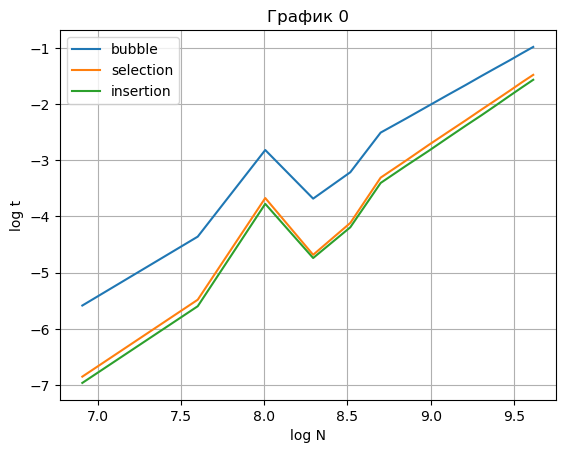
\includegraphics[width=0.75\textwidth]{Assets/graph0.png}
    \caption{log - натуральный логарифм, t - время работы в наносекундах, N - количество элементов}
\end{figure}

Если действительно $t = C * N ^ 2$, то $log t = log C + 2 * log N$. Заметим, что не считая области с $log N = 8$ ($N \approx 2000$) график представляет собой прямую. Посчитаем угловой коэффицент:
\begin{align*}
x &= log N & (x1, y1) &= (7, -7) \\
y &= log t & (x2, y2) &= (9.5, -2)
\end{align*}
\[a = \frac{dy}{dx} = \frac{y2 - y1}{x2 - x1} = \frac{5}{2.5} = 2 \]
Ч.Т.Д, также из графика можно заметить, что selection и insertion имеют гораздо меньший коэффицент С, а значит и работают быстрее
\section{Сравнение Python и C++}
Напишем копию сортировок bubble и insertion на python и сравним в тех же координатах графики:
\begin{figure}[H]
    \centering
    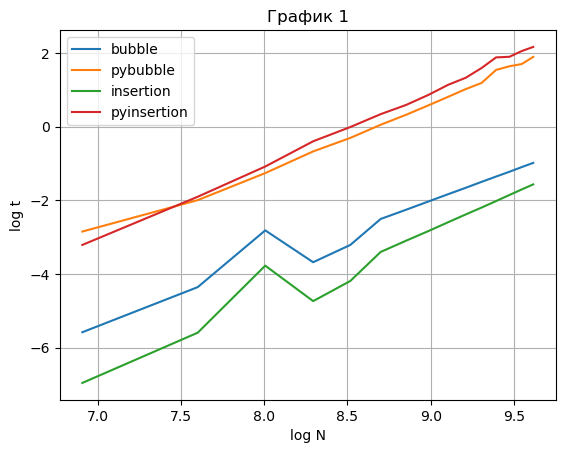
\includegraphics[width=0.75\textwidth]{Assets/graph1.png}
\end{figure}

Время работы отличается почти в $e$ раз, а пик "проблем" приходится на $log N = 9.4$ ($N \approx 12000$)
\section{Оптимизация компилятора}

Предыдущие значения были получены при -О0, добавим другие флаги для сравнения влияния оптимизации компилятора на примере bubble:
\begin{figure}[H]
    \centering
    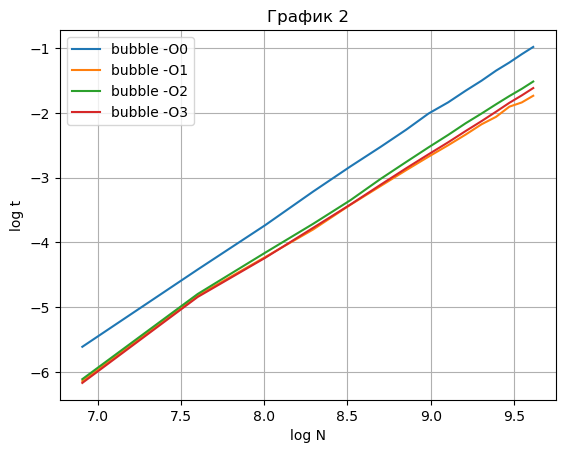
\includegraphics[width=0.75\textwidth]{Assets/graph2.png}
\end{figure}

Переход на -О1 значительно ускорил сортировку, а дальнейшие почти не влияют при выбранном диапазоне (1000 - 20000)
\section{Быстрые сортировки}

Докажим асимптотику $O(NlogN)$ для быстрых сортировок:
\begin{figure}[H]
    \centering
    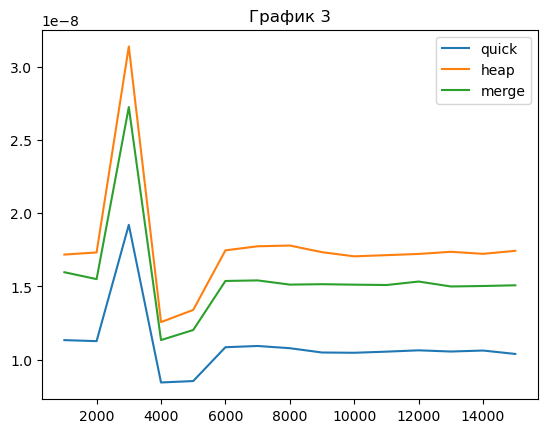
\includegraphics[width=0.75\textwidth]{Assets/graph3.png}
    \caption{По оси ординат $\frac{t}{NlogN}$, по оси абцисс $N$}
\end{figure}

Так как $\frac{t}{NlogN}$ примерно равно 1, то для быстрых сортировок действительно асимптотика $O(NlogN)$.
Заметим также, что в наличии "проблемный" пик около 3000
\section{$O(N^2)$ vs $O(N*logN)$}

Сравним сортировки с разной асимптотикой:
\begin{figure}[H]
    \centering
    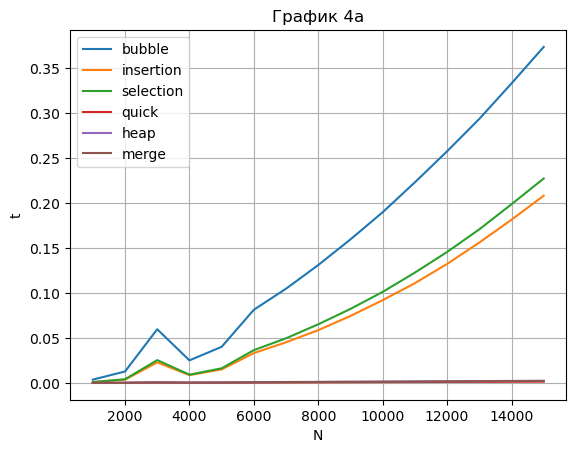
\includegraphics[width=0.75\textwidth]{Assets/graph4a.png}
\end{figure}

$O(N*logN)$ во много раз быстрее на больших размерах массива
\section{Начальные значения}
Теперь исследуем как меняется асимптотика в зависимости от начального массива у разных сортировок
\begin{figure}[H]
    \centering
    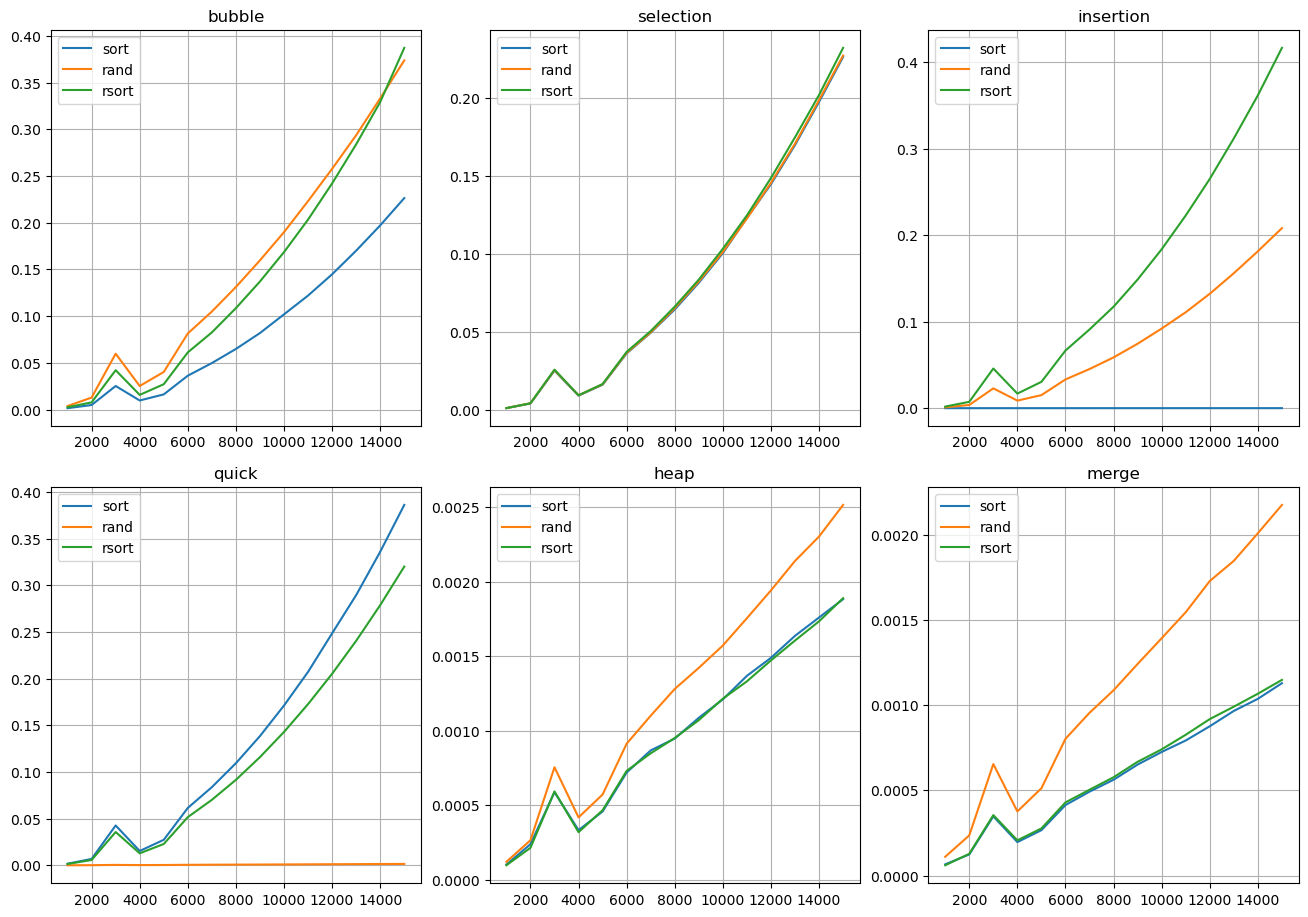
\includegraphics[width=1.1\textwidth]{Assets/graph5.png}
    \caption{sort - отсортированный массив, rand - рандомные значения, rsort - массив отсортированный в обратном порядке}
\end{figure}
Быстрые сортировки имеют схожую асимптотику для сортированных массивов. Selection неважно какой массив, асимптотика почти одинаковая
\section{Малые массивы}
Асимптотика для малых значений, точность составляет 70 измерений на одно количество элементов
\begin{figure}[H]
    \centering
    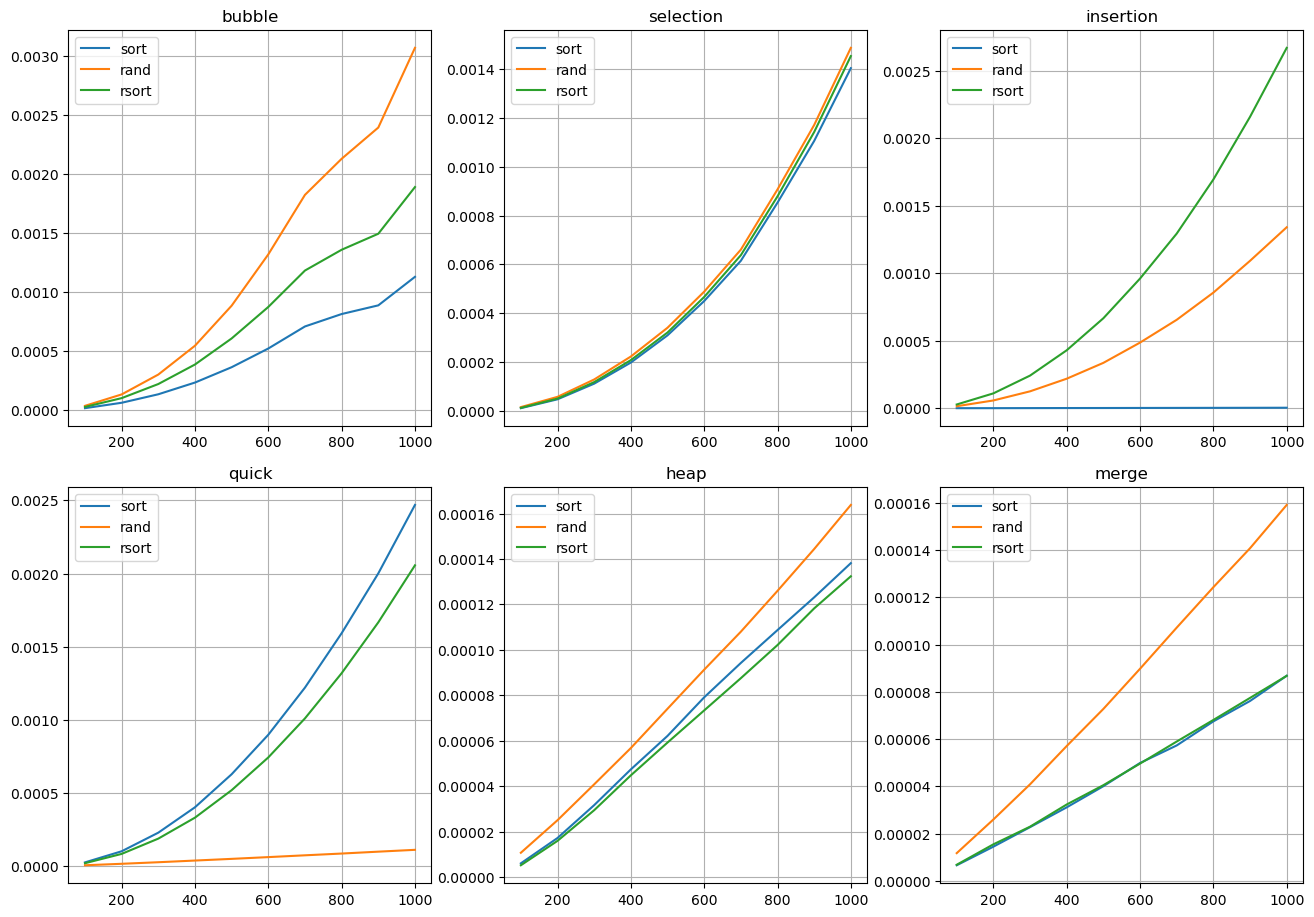
\includegraphics[width=1.1\textwidth]{Assets/graph6.png}
\end{figure}
Благодаря точности графики получились очень гладкими, заметные изменения только у bubble
\section{Тип данных}
Для исследования зависимости асимпототики от типа значений массива в helper.hpp создана "тяжелая" структура, содержащая 100 значений int. 
\begin{figure}[H]
    \centering
    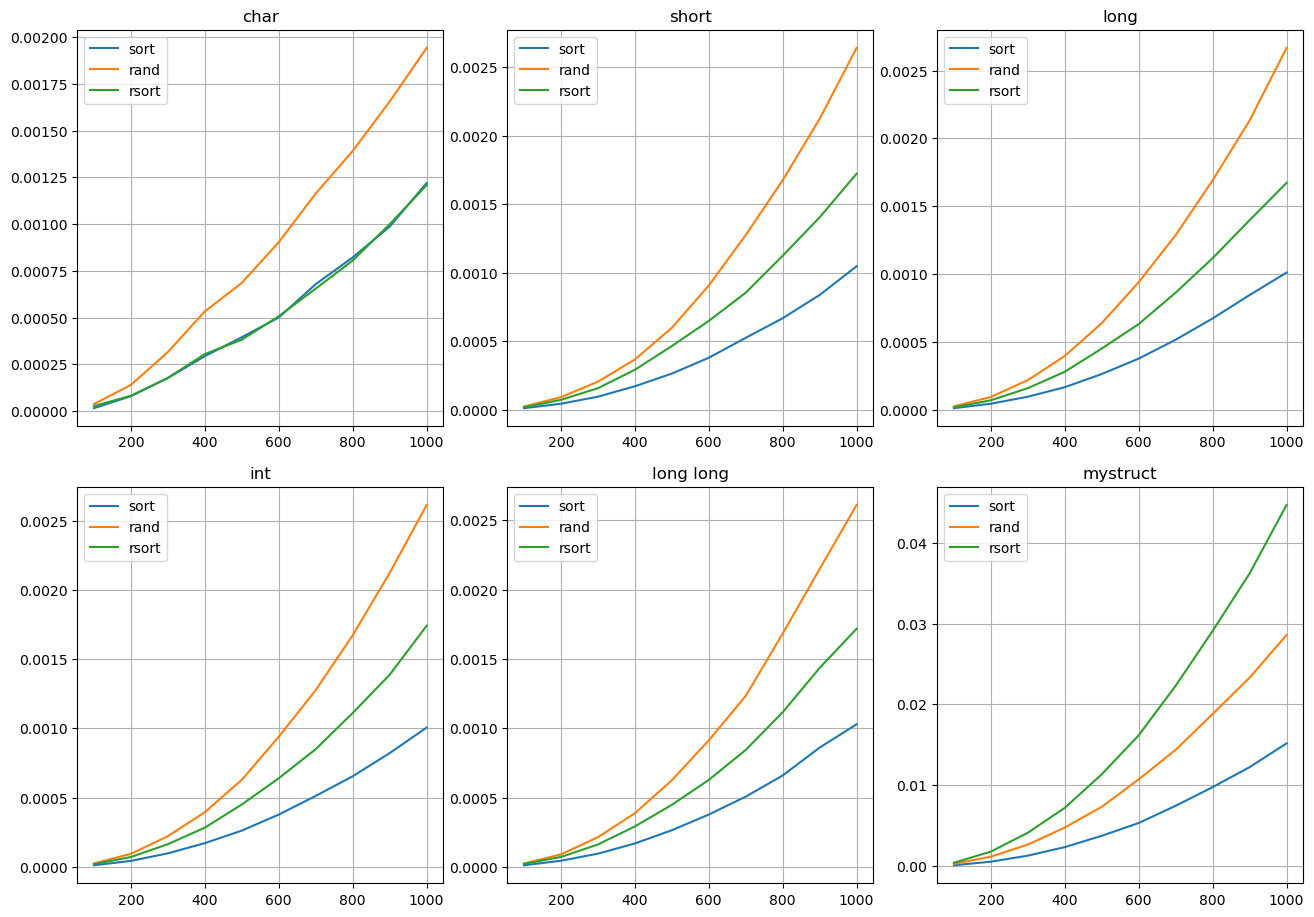
\includegraphics[width=1\textwidth]{Assets/graph7.png}
    \caption{Используется сортировка bubble для малых размеров массива}
\end{figure}
Чем меньше "вес" структуры, тем на порядок быстрее происходит сортировка, это связано с процессом копирования её значений, в теории, если хранить только указатели на значения, то асимптотика будет примерно одинаковой. 
\begin{figure}[H]
    \centering
    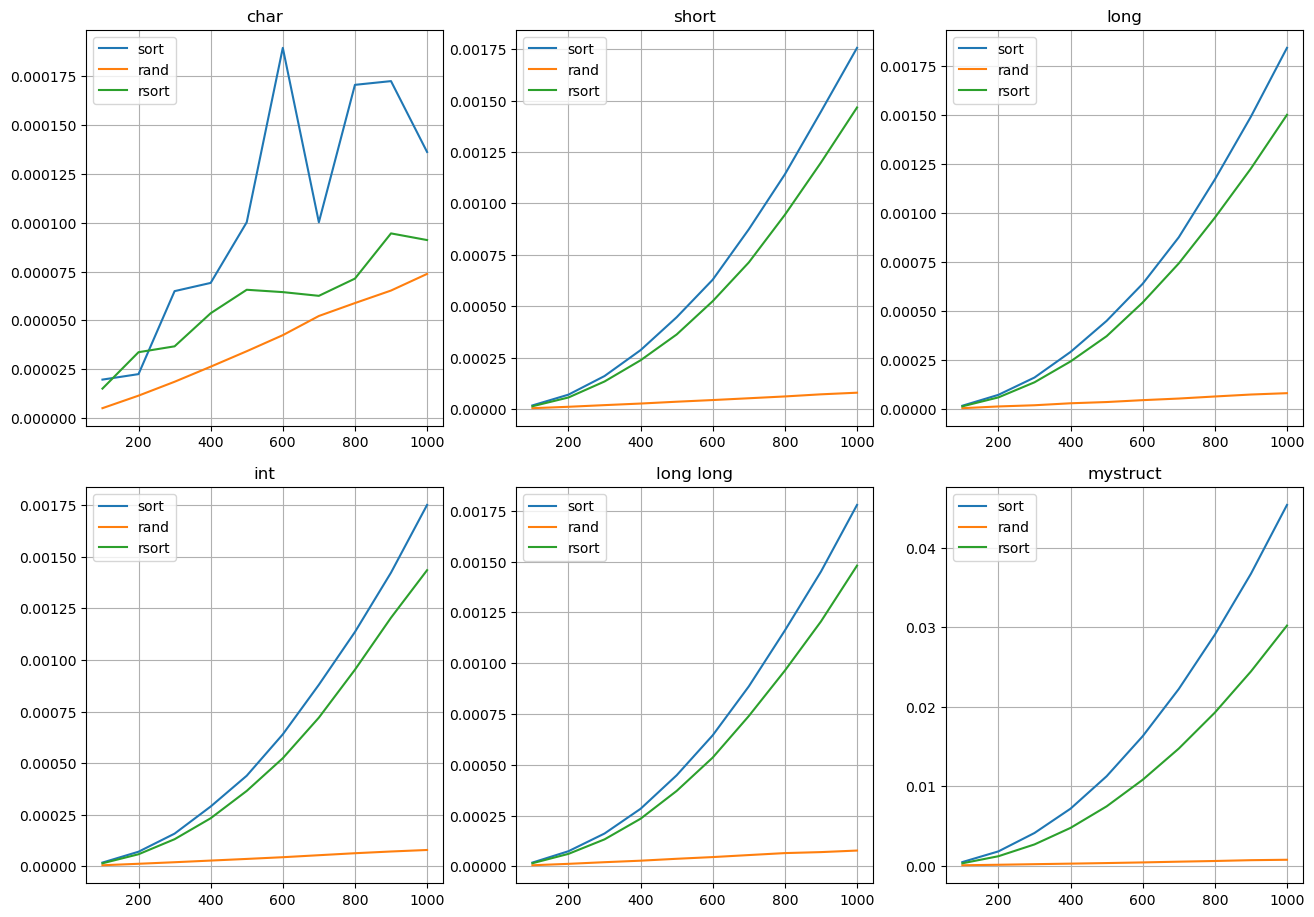
\includegraphics[width=1\textwidth]{Assets/graph8.png}
    \caption{Используется сортировка quick для малых размеров массива}
\end{figure}
Char имеет негладкую асимптотику, что связано со сверхнизким временем работы, несмотря на точность. В целом график асимптотики схожий, отличается только порядок времени работы.
\section{Выводы}
\begin{enumerate}
    \item Python медленее С++
    \item Временная сложность соответствует асимптотике почти на всем диапазоне размеров массивов
    \item Оптимизация компилятора ускоряет работу при -О1, дальнейшим ускорением можно пренебречь
    \item Разные сортировки имеют разную асимптотику при отсортированном, рандомным и отсортированном в обратной последовательности массивах. Кроме selection.
    \item "Вес"\hspace{3pt}типа элементов существенно влияет на время сортировки
\end{enumerate}
\end{document}